\documentclass[]{article}
\usepackage{lmodern}
\usepackage{amssymb,amsmath}
\usepackage{ifxetex,ifluatex}
\usepackage{fixltx2e} % provides \textsubscript
\ifnum 0\ifxetex 1\fi\ifluatex 1\fi=0 % if pdftex
  \usepackage[T1]{fontenc}
  \usepackage[utf8]{inputenc}
\else % if luatex or xelatex
  \ifxetex
    \usepackage{mathspec}
  \else
    \usepackage{fontspec}
  \fi
  \defaultfontfeatures{Ligatures=TeX,Scale=MatchLowercase}
\fi
% use upquote if available, for straight quotes in verbatim environments
\IfFileExists{upquote.sty}{\usepackage{upquote}}{}
% use microtype if available
\IfFileExists{microtype.sty}{%
\usepackage{microtype}
\UseMicrotypeSet[protrusion]{basicmath} % disable protrusion for tt fonts
}{}
\usepackage[margin=1in]{geometry}
\usepackage{hyperref}
\hypersetup{unicode=true,
            pdftitle={California Water Rate Survey Results 2017},
            pdfborder={0 0 0},
            breaklinks=true}
\urlstyle{same}  % don't use monospace font for urls
\usepackage{graphicx,grffile}
\makeatletter
\def\maxwidth{\ifdim\Gin@nat@width>\linewidth\linewidth\else\Gin@nat@width\fi}
\def\maxheight{\ifdim\Gin@nat@height>\textheight\textheight\else\Gin@nat@height\fi}
\makeatother
% Scale images if necessary, so that they will not overflow the page
% margins by default, and it is still possible to overwrite the defaults
% using explicit options in \includegraphics[width, height, ...]{}
\setkeys{Gin}{width=\maxwidth,height=\maxheight,keepaspectratio}
\IfFileExists{parskip.sty}{%
\usepackage{parskip}
}{% else
\setlength{\parindent}{0pt}
\setlength{\parskip}{6pt plus 2pt minus 1pt}
}
\setlength{\emergencystretch}{3em}  % prevent overfull lines
\providecommand{\tightlist}{%
  \setlength{\itemsep}{0pt}\setlength{\parskip}{0pt}}
\setcounter{secnumdepth}{0}
% Redefines (sub)paragraphs to behave more like sections
\ifx\paragraph\undefined\else
\let\oldparagraph\paragraph
\renewcommand{\paragraph}[1]{\oldparagraph{#1}\mbox{}}
\fi
\ifx\subparagraph\undefined\else
\let\oldsubparagraph\subparagraph
\renewcommand{\subparagraph}[1]{\oldsubparagraph{#1}\mbox{}}
\fi

%%% Use protect on footnotes to avoid problems with footnotes in titles
\let\rmarkdownfootnote\footnote%
\def\footnote{\protect\rmarkdownfootnote}

%%% Change title format to be more compact
\usepackage{titling}

% Create subtitle command for use in maketitle
\newcommand{\subtitle}[1]{
  \posttitle{
    \begin{center}\large#1\end{center}
    }
}

\setlength{\droptitle}{-2em}
  \title{California Water Rate Survey Results 2017}
  \pretitle{\vspace{\droptitle}\centering\huge}
  \posttitle{\par}
  \author{}
  \preauthor{}\postauthor{}
  \date{}
  \predate{}\postdate{}


\begin{document}
\maketitle

\section{Introduction}\label{introduction}

The \href{http://californiadatacollaborative.org/}{California Data
Collaborative (``CaDC'')} is a coalition of water utilities that have
pioneered a new data infrastructure non-profit 501 (c) (3) to support
water managers in meeting their reliability objectives and serve the
public good.

One important contribution of the CaDC was to establish a standard
format and to provide the infrastructure for storage and maintainance of
an open database for water rates, facilitating the work of analysts,
economists and software developers interested in analyzing and
understanding the differences in water rate structures and prices across
many different agencies and locations. The water rate structures were
organized in
\href{https://github.com/California-Data-Collaborative/Open-Water-Rate-Specification}{Open-Water-Rate-Specification
(OWRS)} files, a format based on \href{http://yaml.org/}{YAML}, which is
designed to be easy to store, transmit, and parse in any programming
language while also being easy for humans to read.

This report presents a summary of the types of analyses and insights
that can be obtained from analyzing the OWRS, especially when this
information is combined with the water consumption data from water
agencies and Census Data.

\section{Data}\label{data}

This report provides the combined analysis of data from 4 different
sources:

\begin{itemize}
\tightlist
\item
  Water Rates from the
  \href{https://github.com/California-Data-Collaborative/Open-Water-Rate-Specification}{Open-Water-Rates-Specification}.
\item
  Water Consumption data reported by the water agencies {[}ADD MORE
  DETAIL{]}
\item
  Demographic Data from the American Community Survey {[}??{]}
\item
  Qualitative Data from a Survey realized by the California Data
  Collaborative with water agencies in 2017.
\end{itemize}

\section{Summary Statistics}\label{summary-statistics}

This section discusses general characteristics of the rates for
utilities analyzed in this survey.

\begin{figure}
\centering
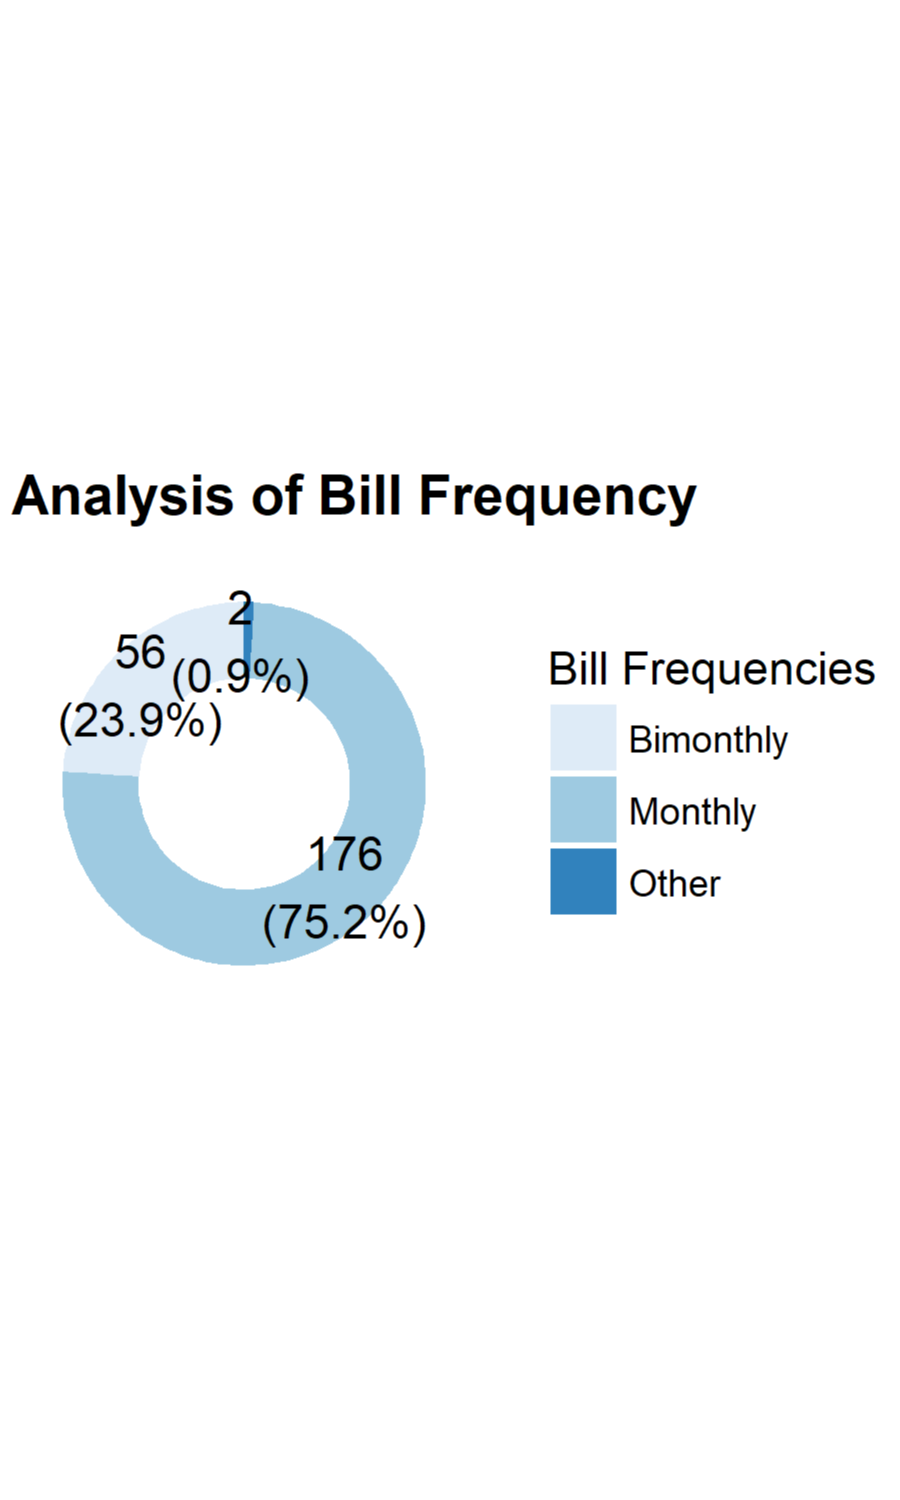
\includegraphics{owrs_analysis_files/figure-latex/bill_frequency_pie-1.pdf}
\caption{Figure 1: Bill Frequency Pie Chart. About three quarters of the
water agencies use a monthly billing system.}
\end{figure}

\begin{figure}
\centering
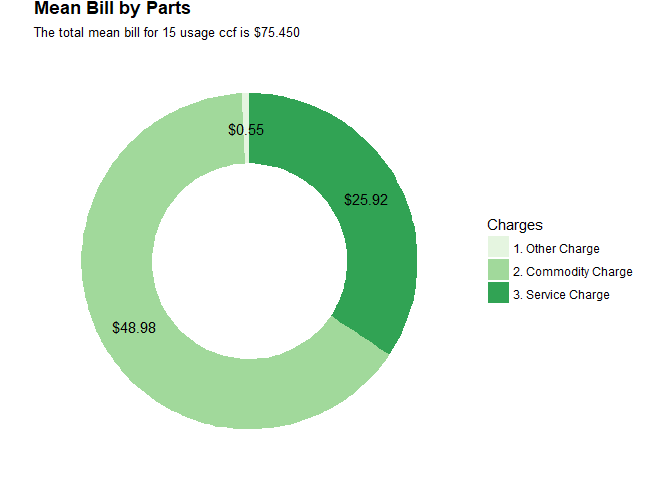
\includegraphics{owrs_analysis_files/figure-latex/mean_bill_by_parts_pie-1.pdf}
\caption{Figure 2: Average bill by parts for all agencies, considering a
consumption of 10 CCF in a month. The average total bill is \$60.68.
With an average service charge (fixed) of \$24.63 (40.6\%) and an
average commodity charge (variable) of \$35.61 (58.7\%).}
\end{figure}

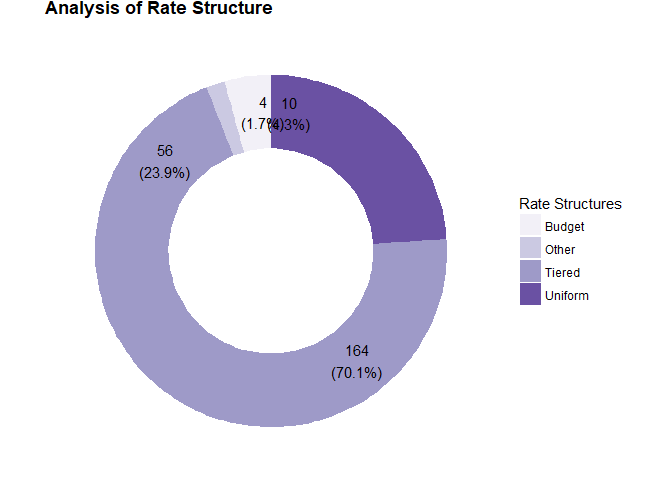
\includegraphics{owrs_analysis_files/figure-latex/rate_structure_type_pie-1.pdf}

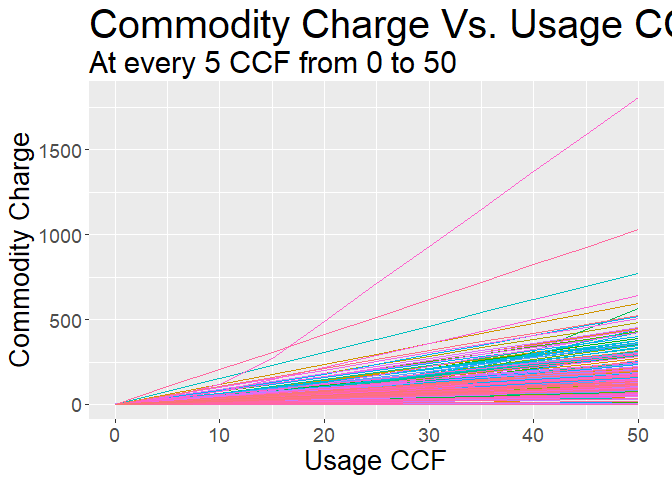
\includegraphics{owrs_analysis_files/figure-latex/commodity_charge_vs_usage_line-1.pdf}

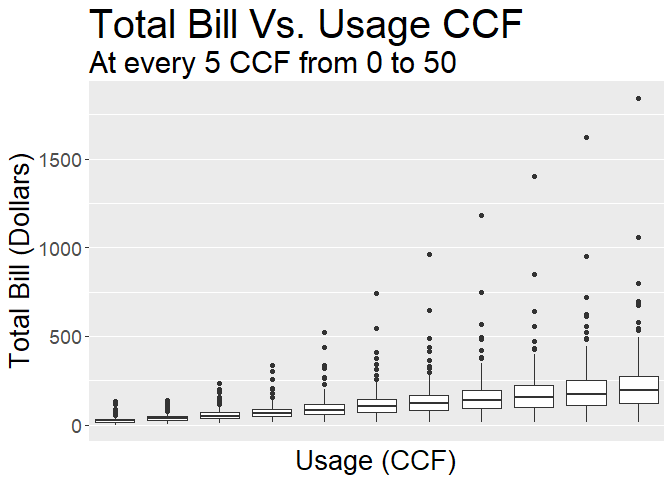
\includegraphics{owrs_analysis_files/figure-latex/commodity_charge_vs_usage_boxplot-1.pdf}

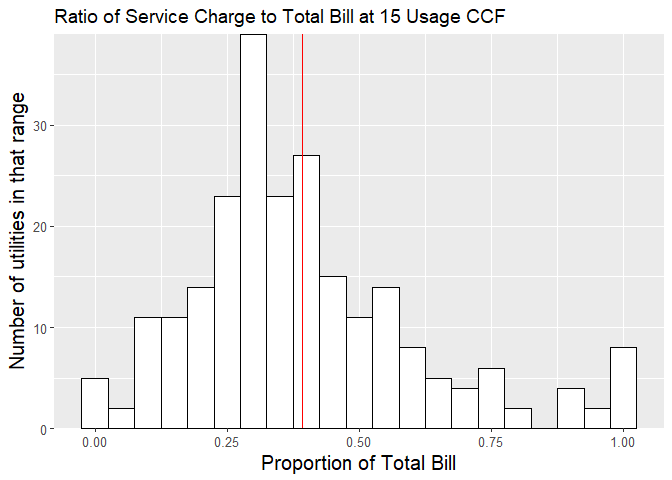
\includegraphics{owrs_analysis_files/figure-latex/service_charge_ratio_histogram-1.pdf}

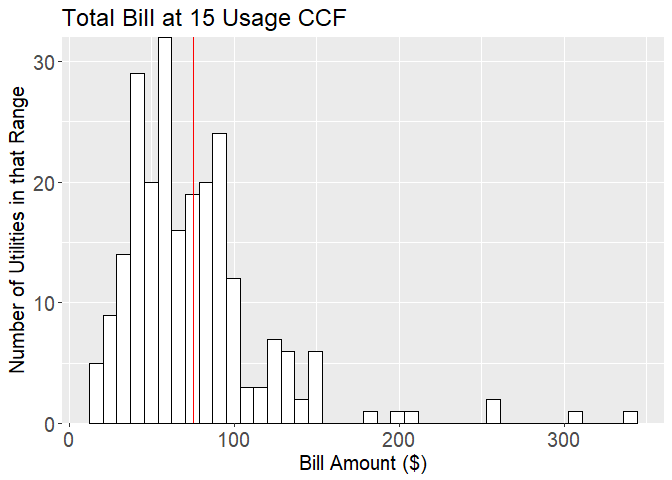
\includegraphics{owrs_analysis_files/figure-latex/total_bill_histogram-1.pdf}

\section{Rates x Efficiency}\label{rates-x-efficiency}

\subsection{Define Period of Analysis}\label{define-period-of-analysis}

Average water rates history:

\subsection{Calculate Efficiency}\label{calculate-efficiency}

Load suppliers report info and join with the Utilities list from the
OWRS files

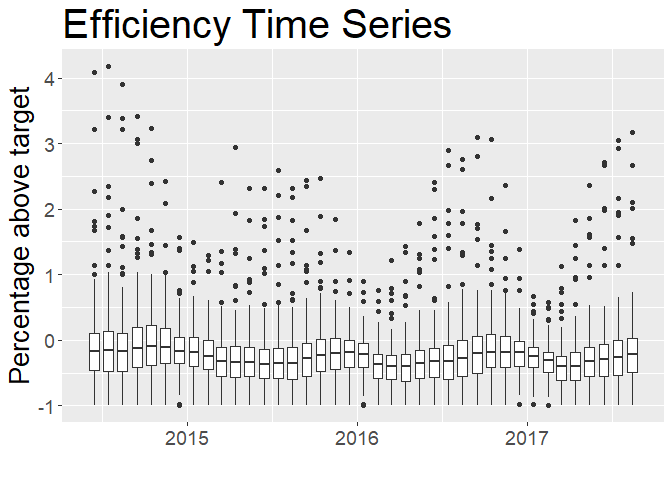
\includegraphics{owrs_analysis_files/figure-latex/efficiency_goal_time_series_boxplot-1.pdf}

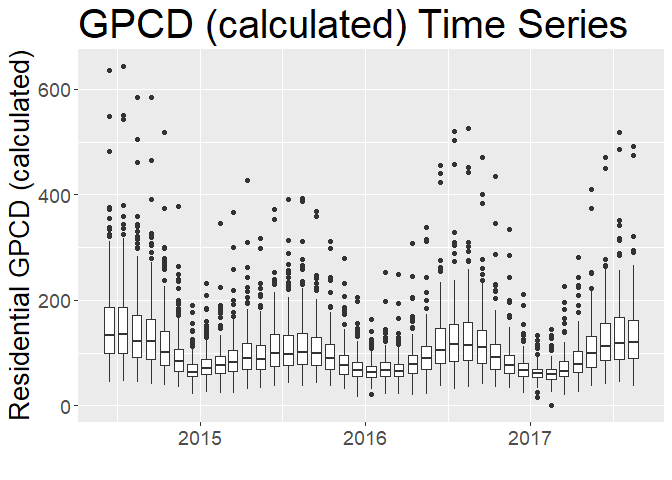
\includegraphics{owrs_analysis_files/figure-latex/gpcd_time_series_boxplot-1.pdf}
\#\# Compare Rates and efficiency

\begin{verbatim}
## Warning in `[<-.data.frame`(`*tmp*`, new_name_column, value =
## list(c("Alameda County Water District", : provided 2574 variables to
## replace 1 variables
\end{verbatim}

Scatter plot of Efficiency (pct\_above\_target) vs Rates (Total Bill for
15 CCF)
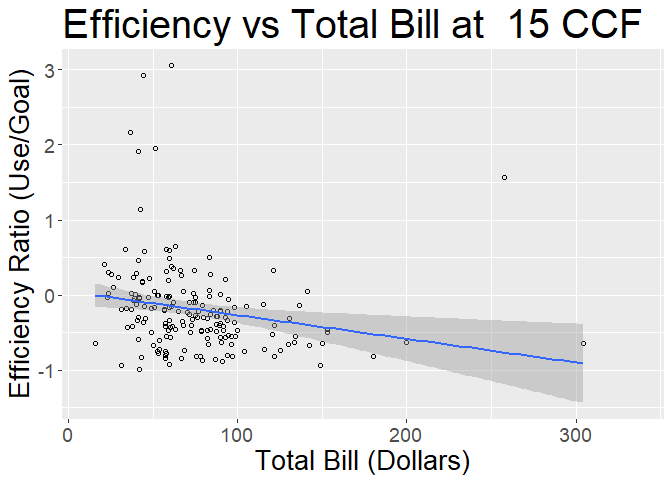
\includegraphics{owrs_analysis_files/figure-latex/efficiency_goal_vs_total_bill_scatter_trend-1.pdf}

\subsection{Joining Data from the Qualitative
Survey}\label{joining-data-from-the-qualitative-survey}

\begin{verbatim}
## Warning: NAs introduced by coercion

## Warning: NAs introduced by coercion
\end{verbatim}

Scatter plot of Efficiency vs Rates Structure (\% Fixed - for 15 CCF)
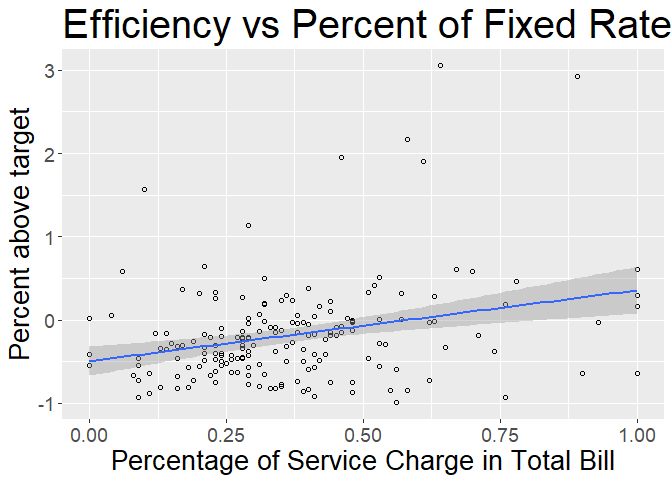
\includegraphics{owrs_analysis_files/figure-latex/efficiency_goal_vs_percent_fixed_scatter_trend-1.pdf}

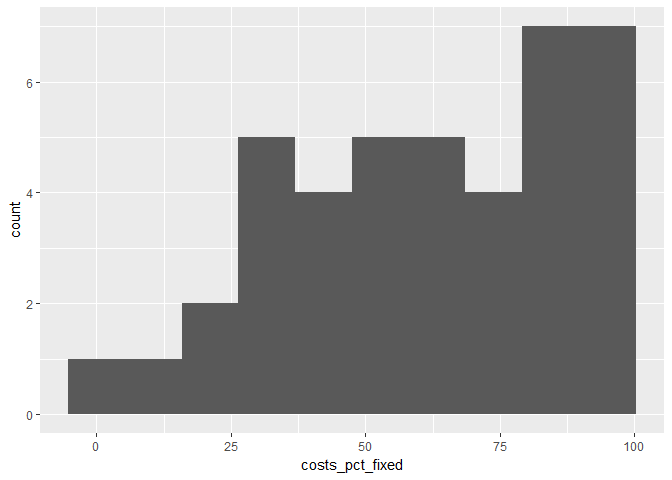
\includegraphics{owrs_analysis_files/figure-latex/fixed_cost_percentage_histogram-1.pdf}

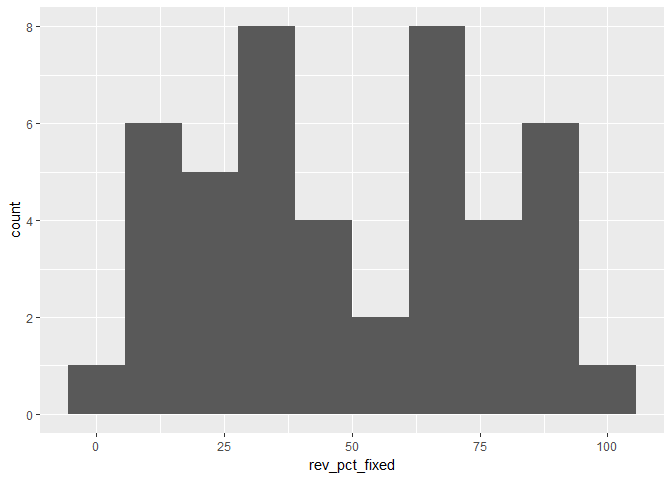
\includegraphics{owrs_analysis_files/figure-latex/fixed_revenue_percentage_histogram-1.pdf}

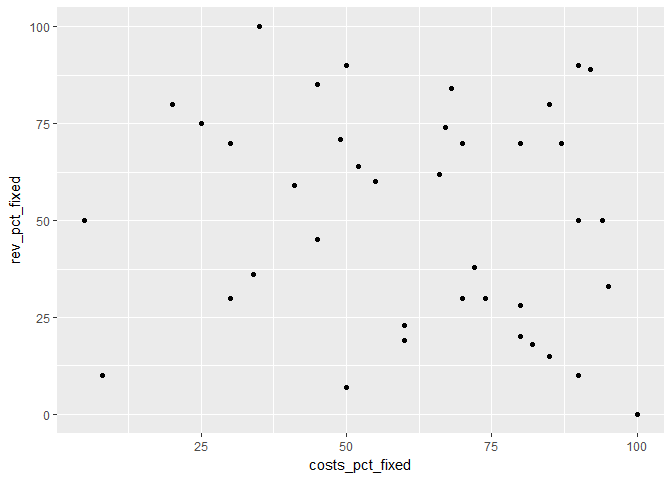
\includegraphics{owrs_analysis_files/figure-latex/fixed_costs_vs_fixed_rev_scatter-1.pdf}


\end{document}
